
RS232IF klassen er blevet testet for at vi kunne være sikre på at kommunikationen imellem PC og CSS-hovedenheden forløb som den skulle. Klassen skal kunne sende kommandoer, til aktiver og deaktiver og spørge CSS-hovedenheden om der stadig er logget ind. Derudover skal den kunne læse 3 forskellige beskeder som hovedenheden kan finde på at sende. Babyalarm, login og login udløbet. I test programmet er der oprettet en metode som kan sende de kald som CSS-hovedenheden ville sende for at simulere det. Der testes så på om metoden read læser og returnere det rigtige. 

\medskip

Testen foregår ved at man laver et loop back ved hjælp af et STK500-kit. Loop-backet gør at det jeg sender bliver returnere, på den måde kan man kontrollere både at det der bliver sendt er korrekt men også at returværdierne for read-metoden er korrekte. 

\medskip

STK500-kittet kobles til computeren hvor test programmet ligger. Der benyttes STK500-kittes "SPARE-port". Der kontrolleres at den port man har valgt på computeren er port 4 (defineret i programmet) ellers skal man ind i RS232IF headeren hvor port er defineret, og ændre det til den korrekt port. Derefter forbinder man TX og RX på STK500-kittet for at skabe loop-back
 
 \medskip
Efter programmet er kørt, kan man på skærmen se hvad der blev sendt, hvilken værdi read forventes at returnere, hvad der blev læst og hvilken værdi read returnerede.

\begin{figure}[!htb]
     {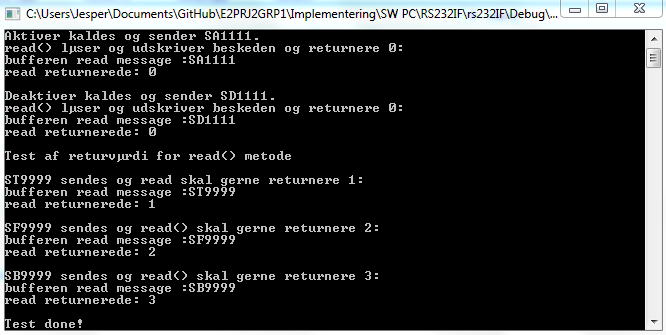
\includegraphics[width=\textwidth]{billeder/SWTest/RS232IF_pc_test}}
     \caption{test af RS232IF klassen via loop-back}
     \label{fig:RS232IF klasse test}
\end{figure}